% 2016 全国卷Ⅰ理科第 24 题：作图用直角坐标网格。
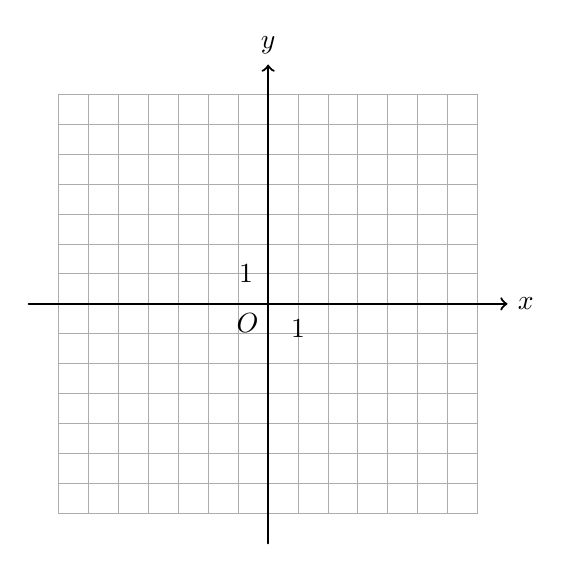
\begin{tikzpicture}[x=0.38cm,y=0.38cm,line cap=round,line join=round]
\foreach \x in {-7,-6,...,7} {
  \draw[gray!65,line width=0.35pt] (\x,-7) -- (\x,7);
}
\foreach \y in {-7,-6,...,7} {
  \draw[gray!65,line width=0.35pt] (-7,\y) -- (7,\y);
}
\draw[->,thick] (-8,0) -- (8,0) node[right] {$x$};
\draw[->,thick] (0,-8) -- (0,8) node[above] {$y$};
\node[below left] at (0,0) {$O$};
\node[left=2pt] at (0,1) {$1$};
\node[below=2pt] at (1,0) {$1$};
\end{tikzpicture}
